\documentclass{article}
\usepackage[utf8]{inputenc}
\usepackage[english, swedish]{babel}

\usepackage{cite}
\usepackage{caption}
\usepackage{graphicx}
\usepackage{float}
\usepackage{textcomp}

\usepackage{listings}
\usepackage{color}
 
\definecolor{codegreen}{rgb}{0,0.6,0}
\definecolor{codegray}{rgb}{0.5,0.5,0.5}
\definecolor{codepurple}{rgb}{0.58,0,0.82}
\definecolor{backcolour}{rgb}{0.95,0.95,0.92}
 
\lstdefinestyle{mystyle}{
    backgroundcolor=\color{backcolour},   
    commentstyle=\color{codegreen},
    keywordstyle=\color{magenta},
    numberstyle=\tiny\color{codegray},
    stringstyle=\color{codepurple},
    basicstyle=\footnotesize,
    breakatwhitespace=false,         
    breaklines=true,                 
    captionpos=b,                    
    keepspaces=true,                 
    numbers=left,                    
    numbersep=5pt,                  
    showspaces=false,                
    showstringspaces=false,
    showtabs=false,                  
    tabsize=2
}

\lstset{style=mystyle}

\usepackage[yyyymmdd]{datetime}
\renewcommand{\dateseparator}{-}

\usepackage{graphicx}
\graphicspath{ {images/} }

%For headers & footers
\usepackage{fancyhdr}
\pagestyle{fancy}
\lhead{
\includegraphics[scale=0.2]{Logo}}
\chead{Kartrobot}
\rhead{\today}

\lfoot{Konstruktion med mikrodatorer}
\rfoot{Grupp 3}

\usepackage{titlesec}

\setcounter{secnumdepth}{4}

\titleformat{\paragraph}
{\normalfont\normalsize\bfseries}{\theparagraph}{1em}{}
\titlespacing*{\paragraph}
{0pt}{3.25ex plus 1ex minus .2ex}{1.5ex plus .2ex}

\renewcommand{\headrulewidth}{0.4pt}
\renewcommand{\footrulewidth}{0.4pt}


\title{Efterstudie}
\author{Patrik Sletmo}
\date{\today}

\selectlanguage{swedish}

\begin{document}

\thispagestyle{empty}

{
\sffamily
\centering
\large


{\huge 
Efterstudie
}

{\large
Patrik Sletmo
}

{\large
Version 1.0
}

\vspace{3.5cm}

Status
\begin{table}[H]
\centering
\begin{tabular}{ | c | c | c | }
\hline
-- & Patrik Sletmo & 2016-12-XX \\
\hline
\end{tabular}
\end{table}
}
\clearpage

\vspace*{\fill}
{
\sffamily
\centering
\large


{\huge
Projektidentitet
}

{\large
Grupp 3, 16/HT, KarToffel \\ Linköpings tekniska högskola, ISY
}

\vspace{0.5cm}

\begin{table}[H]
\centering
\begin{tabular}{ | c | c | c | c |}
\hline
Namn & Ansvar & Telefon & E-post \\
\hline
Patrik Sletmo & Projektledare & 070 783 57 61 & patsl736@student.liu.se \\
\hline
Rebecca Lindblom & Utvecklare & 073 436 40 79 & rebli156@student.liu.se \\
\hline
Matildha Sjöstedt & Utvecklare & 070 515 84 11 & matsj696@student.liu.se \\
\hline
Sebastian Callh & Utvecklare & 073 820 46 64 & sebca553@student.liu.se \\
\hline
Anton Dalgren & Utvecklare & 076 836 51 56 & antda685@student.liu.se \\
\hline
Matilda Dahlström & Utvecklare & 070 636 33 52 & matda715@student.liu.se \\
\hline
\end{tabular}
\end{table}
}

\begin{center}
\textbf{Hemsida}: https://github.com/SebastianCallh/kartoffel-tsea29
\end{center}

\begin{center}
\textbf{Kund}: Mattias Krysander, 013 - 28 2198 , matkr@isy.liu.se
\end{center}

\begin{center}
\textbf{Kursansvarig}: Tomas Svensson, 3B 528, +46 (0)13 28 1368, tomas.svensson@liu.se \\
\textbf{Handledare}: Anders Nilsson, 3B 512, +46 (0)13 28 2635, anders.p.nilsson@liu.se
\end{center}
\vspace*{\fill}
\clearpage

\renewcommand*\contentsname{Innehållsförteckning}
\tableofcontents

\clearpage
\section{Tidsåtgång}
Text


\subsection{Arbetsfördelning}
Under projektets tidiga skede då vi byggde upp hårdvaran delades arbetet in i de olika delsystemen (huvudenhet, sensorenhet, styrenhet) vilka arbetades på i par om två. Allt eftersom projektet fortskred övergick arbetet främst till att skriva Python-kod på huvudenheten och arbetet delades då in i olika mjukvarumoduler. Vem som gjort vad har genom hela projektet styrts av intresse och kompetens.


\subsection{Tidsåtgång jämfört med planerad tid}
Arbetet med designspecen innan BP3 gick betydligt snabbare än planerat vilket gav oss mer tid inför BP5. Tidsåtgången för själva konstruktionen underskattades dock.

\begin{table}[H]
\centering
\caption{En tabell över projektets tidsåtgång.}
\begin{tabular}{ | c | c | c | }
\hline
Fas & Planerad tid i timmar & Använd tid i timmar \\
\hline
Före & 83 & 52 \\
\hline
Under & 851 & 922 \\
\hline
Efter & 26 & ?? \\
\hline
\end{tabular}
\label{table:tidsatgang}
\end{table}
\ \\


\clearpage
\section{Analys av arbete och problem}
Under konstruktionens inledande fas arbetade gruppen i väldigt separerade grupper med olika implementationer. Arbetet gick under den här perioden bra, men när olika funktionalitet skulle integreras uppstod problem och tiden spenderad på felsökning ökade markant. Efter att gruppen lyckats integrera all funktionalitet spenderades även en signifikant del av den återstående tiden med att testa olika värden på hur vi filtrerade sensorvärden och på att finslipa regleringen. Det var ibland svårt att få perspektiv på hur ändringarna som gjordes skulle påverka robotens prestation, men efter en tid så löste även det problemet sig.

\subsection{Vad hände under de olika faserna (bra/dåligt/orsak)?}
I före-fasen flöt arbetet på bra, men interna deadlines innan de faktiska. Sjukdom påverkade arbetet negativt, men gruppen levererade ändå enligt plan. När under-fasen väl startade tilltog gruppens entusiasm då fokus flyttades från att skriva dokumentation till att vira och koda. Den här entusiasmen höll i sig fram till det att uppstod problem med integration av olika undergruppers moduler, då stämningen försämdares avsevärt. Främst på grund av dålig kommunikation vilket gjorde integrationen svårare än den hade behövt vara. Efter en lyckad leverans lades endast tid på att sammanställa detta dokument.

\subsection{Hur vi arbetade tillsammans (ansvar, beslut, kommunikation etc.)?}
Text

\subsection{Hur använde vi projektmodellen?}
Text

\subsection{Hur fungerade relationen med beställaren?}
Gruppen upplever inte att den haft någon nära relation med beställaren, men att han varit lätt att få tag på och att kommunikationen har fungerat väl. Kritiken som gavs på den tekniska dokumentationen uppskattades. 

\subsection{Hur fungerade relationen med handledaren?}
Handledaren fanns oftast till hands när vi behövde ställa frågor, vilket var en användbar resurs då gruppen konstruerade hårdvaran. Gruppen upplevde inte ett så stort behov att att ställa frågor, men är mycket nöjd med den hjälp som givits.

\subsection{Tekniska framgångar/Problem}

\subsubsection{1. Svårat problem}
\subsubsection{2. Nästa svårast}
\subsubsection{3. Tredje svårast}

\subsubsection{Mätvärden från laser}
Vid första leveransen upplevdes inte positionsbestämningen fungerar konsekvent, vilket visade sig bero på två olika saker. 
\begin{figure}[H]
\centering
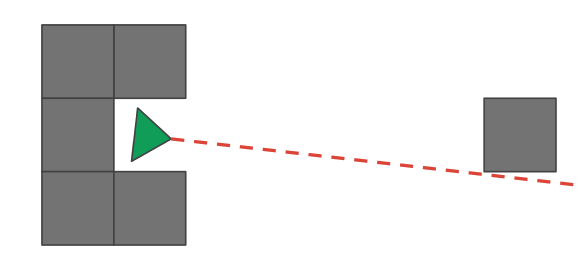
\includegraphics[scale=0.5]{wrongly_positioned_laser}
\caption{En bild på hur fel positionering påverkar lasern.}
\label{fig:wrongly_positioned_laser}
\end{figure}
\ \\
För det första kunde robotens lasersensor ge orimliga värden helt spontant och för det andra så positionerades den inte korrekt efter svängar, vilket ledde till att den på längre avstånd kunde får markanta felläsningar. Se figur~\ref{fig:wrongly_positioned_laser} för en illustration på detta.
\\
Att lasersensorn kunde ge konstiga värden berodde förmodligen på något fel på låg nivå, antingen på robotens I2C-buss eller till och med hårdvara. Detta felsöktes dock inte eftersom det uppskattades ta för lång tid, och fokus lades på att filtrera laservärden på ett sätt som skulle eliminera dessa felaktiga mätningar. Detta gjordes främst genom att ignorera laservärden som skiljde sig för mycket från tidgare värden. Om felet ej hade uppstått hade flertalet dagar kunnat sparas in under projektets sista veckor.
\\
Att roboten kunde ställa sig snett berodde på dess navigeringslogik, vilken fick förbättras. Navigationslogiken är programmerad som en tillståndsmaskin, och för att lösa problemet lades ett nytt tillstånd till som roboten går in i efter varje sväng, där den korrigerar sin riktning. På så sätt kunde det säkerställas att roboten alltid stod parallelt med väggen på höger sida efter en sväng och att lasern träffade där den skulle. När problemet väl upptäcks åtgärdades det på bara några timmar, men det hade länge legat och spökat under testkörningar. Det är svårt att urskilja vilket problem som påverkade när, men även det här felet kan ha kostat gruppen flera dagar av felsökning.

Ordning:
Laser
Bluetooth
WiFi

Kandidater:
Bluetooth
Under utvecklingen av mjukvaruklienten samt robotens uppkoppling mot den, upplevdes stor tidsåtgång på dess aktiviteter. Då både server- och klientsidan utvecklades i Python användes biblioteket Pybluez för Bluetoothuppkopplingen. 

Orsaker till att detta problem uppstod var dels att detta bibliotek var otroligt dåligt dokumenterat, ingen tidigare kunskap om nätverksprogrammering eller processhantering i Python, dålig kommunikation inom gruppen för planering av nivån på utvecklingen, 

WiFi (designfel)


Beskriv de 3 besvärligaste problemen som ni har haft under projektet. 
Rangordna problemen där 1 är mest besvärlig i betydelsen tog längst tid att fixa.
Beskriv för varje problem:
a. felets typ - ange t.ex.  hårdvarufel, mjukvarufel, systemintegrationsfel 
b. kort beskrivning av felets symptom 
c. kort beskrivning av felets orsak t.ex. logiskt fel i programmering, timing-fel, glappkontakt, missförstånd av spec., felaktig design. 
d. kort beskrivning av hur ni fixade felet. T.ex. hur ni fixade mjukvarubuggen, fick ny hårdvara, virade om, gick runt problemet.
e. ungefärlig skattning av hur mycket tid som ni ägnade åt felsökningen (dvs. tid som kunde tjänats in om felet inte hade uppstått)


\clearpage
\section{Måluppfyllelese}
text

\subsection{Vad har uppnåtts?}
text

\subsection{Hur fungerade leveransen?}
Kvällen innan BP5-mötet hade roboten konsekvent klarat en bana, men den var helt klart inte konsekvent nog då den vid leverans inte klarade banan en enda gång. En omleverans bokades in tre dagar senare, och på den tiden lyckades gruppen identifiera och lösa felen som lett till robotens inkonsekventa beteende. Vid det andra BP5-mötet klarade roboten fyra av fyra körningar, varav två kördes på en helt okänd bana. Gruppen är mycket nöjd med robotens kvalitet vid leverans.

\subsection{Hur har studiesituationen påverkat projektet?}
Då nästan hela gruppen har haft olika scheman, deltidsarbetat och varit aktiva i tidskrävande studentföreningar har schemaläggning varit en utmaning, och många timmar har lagts på kvällstid och helger. 

\clearpage
\section{Sammanfattning}
text

\subsection{De tre viktigaste erfarenheterna}

Kandidater:
Kommunicera. Log i slack. Alla.
Tänk igenom hur robust funktionaliteten behöver vara. Over-engineera inte. Team-Bluetooth.
Struktur och planering. Arbete med git. Planering är tråkigt men nyttigt!


\subsection{Goda råd till de som ska utföra ett liknande projekt}
Kommunicera mera! Använd versionshantering. Överskatta tidsåtgång.
Att ha kvar på formen 'roboten ska klara 3/3 körningar' är sjukt våghalsigt

\nocite{*}
\bibliography{efterstudie}{}
\bibliographystyle{plain}

\end{document}
